% Options for packages loaded elsewhere
\PassOptionsToPackage{unicode}{hyperref}
\PassOptionsToPackage{hyphens}{url}
\documentclass[
  11pt,
]{article}
\usepackage{xcolor}
\usepackage[margin=1in]{geometry}
\usepackage{amsmath,amssymb}
\setcounter{secnumdepth}{5}
\usepackage{iftex}
\ifPDFTeX
  \usepackage[T1]{fontenc}
  \usepackage[utf8]{inputenc}
  \usepackage{textcomp} % provide euro and other symbols
\else % if luatex or xetex
  \usepackage{unicode-math} % this also loads fontspec
  \defaultfontfeatures{Scale=MatchLowercase}
  \defaultfontfeatures[\rmfamily]{Ligatures=TeX,Scale=1}
\fi
\usepackage{lmodern}
\ifPDFTeX\else
  % xetex/luatex font selection
\fi
% Use upquote if available, for straight quotes in verbatim environments
\IfFileExists{upquote.sty}{\usepackage{upquote}}{}
\IfFileExists{microtype.sty}{% use microtype if available
  \usepackage[]{microtype}
  \UseMicrotypeSet[protrusion]{basicmath} % disable protrusion for tt fonts
}{}
\makeatletter
\@ifundefined{KOMAClassName}{% if non-KOMA class
  \IfFileExists{parskip.sty}{%
    \usepackage{parskip}
  }{% else
    \setlength{\parindent}{0pt}
    \setlength{\parskip}{6pt plus 2pt minus 1pt}}
}{% if KOMA class
  \KOMAoptions{parskip=half}}
\makeatother
\usepackage{longtable,booktabs,array}
\usepackage{calc} % for calculating minipage widths
% Correct order of tables after \paragraph or \subparagraph
\usepackage{etoolbox}
\makeatletter
\patchcmd\longtable{\par}{\if@noskipsec\mbox{}\fi\par}{}{}
\makeatother
% Allow footnotes in longtable head/foot
\IfFileExists{footnotehyper.sty}{\usepackage{footnotehyper}}{\usepackage{footnote}}
\makesavenoteenv{longtable}
\usepackage{graphicx}
\makeatletter
\newsavebox\pandoc@box
\newcommand*\pandocbounded[1]{% scales image to fit in text height/width
  \sbox\pandoc@box{#1}%
  \Gscale@div\@tempa{\textheight}{\dimexpr\ht\pandoc@box+\dp\pandoc@box\relax}%
  \Gscale@div\@tempb{\linewidth}{\wd\pandoc@box}%
  \ifdim\@tempb\p@<\@tempa\p@\let\@tempa\@tempb\fi% select the smaller of both
  \ifdim\@tempa\p@<\p@\scalebox{\@tempa}{\usebox\pandoc@box}%
  \else\usebox{\pandoc@box}%
  \fi%
}
% Set default figure placement to htbp
\def\fps@figure{htbp}
\makeatother
\setlength{\emergencystretch}{3em} % prevent overfull lines
\providecommand{\tightlist}{%
  \setlength{\itemsep}{0pt}\setlength{\parskip}{0pt}}
\usepackage{fancyhdr}
\pagestyle{fancy}
\fancyhead[L]{\textit{Short report title}}
\fancyhead[R]{\leftmark}
\fancyfoot[C]{\thepage}
\usepackage{setspace}
\onehalfspacing
\usepackage{titling}
\pretitle{\begin{center}\LARGE\bfseries}
\posttitle{\end{center}\vspace{1em}}
\usepackage{caption}
\captionsetup[figure]{labelfont=bf,textfont=it}
\captionsetup[table]{labelfont=bf}
\usepackage{titlesec}
\newcommand{\sectionbreak}{\clearpage}
\usepackage{booktabs}
\usepackage{longtable}
\usepackage{array}
\usepackage{multirow}
\usepackage{wrapfig}
\usepackage{float}
\usepackage{colortbl}
\usepackage{pdflscape}
\usepackage{tabu}
\usepackage{threeparttable}
\usepackage{threeparttablex}
\usepackage[normalem]{ulem}
\usepackage{makecell}
\usepackage{xcolor}
\usepackage{bookmark}
\IfFileExists{xurl.sty}{\usepackage{xurl}}{} % add URL line breaks if available
\urlstyle{same}
\hypersetup{
  pdftitle={Report Title: Example Report},
  hidelinks,
  pdfcreator={LaTeX via pandoc}}

\title{Report Title: Example Report}
\author{Group 13\\
Department / Course}
\date{November 17, 2025}

\begin{document}
\maketitle

{
\setcounter{tocdepth}{3}
\tableofcontents
}
\section{Executive Summary}\label{executive-summary}

In the UK it is a criminal offence to drive a motor vehicle with a blood
or breath alcohol concentration above the prescribed limit. When a
person is arrested for driving under the influence of alcohol it is not
usually possible to perform an accurate test of the level of alcohol in
the blood or breath immediately. Breath tests can be used as an initial
screening tool at the scene, but these are not sufficiently accurate for
prosecution. Instead, people are taken to a police station or hospital,
where the test can be carried out using proper laboratory protocols. As
the body clears alcohol from the blood through time this means that if
the individual was over the limit, the measured blood alcohol
concentration (BAC) will be lower at the time of measurement than it was
when the person was driving a motor vehicle. To deal with this
situation, If the BAC after time \(t\) (hours) is measured as \(C_t\)
(g/kg), the BAC at time \(0\) is estimated as \(C_0 = C_t - βt\), where
\(\beta\) (\(g/kg/h\)) is BAC elimination rate.

The key point is how to find a precise \(\beta\) to estimate \(C_0\).
Forensic scientists currently \(2.5\%\) percentile of \(\beta\)
distribution constructing from samples as the estimated \(\beta\) value
for every individuals. This method is obviously not rigorous enough for
the courts, since:

\begin{itemize}
\tightlist
\item
  The courts will be forced to make decisions under estimated \(\beta\)
  if we only give a single estimation of \(beta\), since the calculated
  \(C_0\) is either over or under the legal limit.
\item
  Differences between individuals are ignored, for example age and sex,
  which may affect \(\beta\).
\item
  \(\beta\) value at \(2.5\%\) is over conservative and most
  uncertainties are hiding.
\end{itemize}

In this report, we will introduce a Bayesian regression model with
considering the heterogeneity between individuals, the model gives a
posterior distribution of \(\beta\) by using both samples and prior
knowledge. Then we randomly simulate \(4000\) \(\beta\) values from
posterior distribution and find out the probability of the person's BAC
over limit while driving.

In real world, \(\beta\) estimation is quite difficult, it depends on
the individuals' liver condition, drinking habits, genetic, diet, etc.
As we don't have corresponding data, in our regression model of
\(\beta\) is mainly dominate by gender, but we still find some useful
variables:

\begin{itemize}
\item
  Gender: Female's BAC elimination rate is larger than male on average,
  it is explained by liver weight represents a greater fraction of lean
  body mass in the female gender {[}2{]}.
\item
  Drinking time after BAC peak: If the person keep drinking after BAC
  reaches peak, the measured \(\beta\) will be smaller since \(\beta\)
  is measured starting at BAC peak time till the end, there will be
  fluctuations on the BAC plots.
\end{itemize}

When it is too late to use a blood or breath test and the only
information available is eyewitness testimony of the quantity of alcohol
consumed. We have to use Widmark's equation:
\[C_t = \frac{A}{Weight \times V_d} - \beta t\]

where \(A\) is Amount of Alcohol Consumed (g), \(V_d\) is the volume of
distribution that need to be found. Forensic scientists use the same
method again to estimate \(V_d\) separately with \(\beta\). But \(V_d\)
and \(\beta\) are not independent, so we build a joint Bayesian
regression model, which can simulate them together to solve with the
correlation. Then again after simulation, each \(C_t\) is calculated by
each pair of \(\beta\) and \(V_d\), so expert witness can still find a
probability of \(C_t\) exceeding the limit.

To make it easier, we write the method in a function so other expert
witness can also get the results by easily plugging new person's data.

\section{Data Description}\label{data-description}

It is important to normalized all numerical variables. Centering the
covariates can reduce autocorrelation \(\rho_k\) of lag \(k\) which is
defined as:

\[\rho_k = \frac{Cov(\theta^i, \theta^{i+k})}{\theta^2},\] \(\rho_k\)
measures how similar the sample at position \(i\) is to the sample at
position \(i+k\). As the random walk process, \(\theta_i\) is similar to
\(\theta_{i+1}\), less similar to \(\theta_{i+2}\), independent with
\(\theta_{i+k}\) for large \(k\). So if \(\rho_k\) is large means the
chains hardly move, can't converge.

As a more clear expression, we will introduce Effective Sample Size
(ESS):

\[ n_{\text{eff}} = \frac{n}{1 + 2 \sum_{k=1}^{\infty}\rho_k}\]

\(n_{\text{eff}}\) is larger means the MCMC method converge faster (for
example if we set \(4\) chains with each chains \(2000\) iterations,
\(500\) burn-in, the \(n_{\text{eff}} = 4000\) means the number of
independent samples is \(4000\) out of \(8000\)). Larger
\(n_{\text{eff}}\) in same number of iterations means smaller variance
of estimated exoectation since:

\[\mathrm{V}(\hat{E}(\beta)) \approx \frac{\sigma^2}{n_{\text{eff}}}.\]

Also Since \(\beta\) is a small value, the coefficients of large value
variables are pretty small, near 0, which will make \(\beta\) estimation
worse.

Then we prefer to \(\beta\) to \(\log(\beta)\) since the original
\(\beta\) distribution has heavy tail, all outliers (if have) can be
scaled. As shown in figure 1, \(\beta\) forms a good normal distribution
shape after log-transferring. After simulation we can take exponential
of the results.

`BAC Peak time' is converted to hours.

\begin{figure}
\centering
\pandocbounded{\includegraphics[keepaspectratio]{Untitled_files/figure-latex/unnamed-chunk-2-1.pdf}}
\caption{log(beta) distribution.}
\end{figure}

Since \(\beta\) is a constant rate, measured when the BAC curve reaches
peak and starts to decrease, so variables like AAC and Maximum BAC will
not be used, since they are correlated with the value of BAC, not BAC
elimination rate.

From the dataset, most data comes from age smaller than \(30\)
(\(85/100\)), so even though age is sufficient variable for \(\beta\)
the model can't really recognize it. Research shows that age doesn't
really matter unless the subject has age-related liver disease, but
because of moral and ethical, we don't find much research of alcohol
test on elderly person with liver disease.

\section{Bayesian regression model
(BRM)}\label{bayesian-regression-model-brm}

\subsection{Reason for BRM}\label{reason-for-brm}

Comparing with fitting linear regression model for \(\beta_i\), which
can be expressed as:

\[\hat{\beta}_{i,j} = \hat{\gamma}_{1}\,\text{female}_j
+ \hat{\gamma}_{2}\,\text{male}_j
+ \hat{\gamma}_{3}\,\text{weight}_j
+ \hat{\gamma}_{4}\,\text{height}_j + \sigma^2_i\]

and giving a exact value of \(\hat{\beta_i}\) for \(i_{th}\) estimation
of \(\hat{\beta}\) under \(\sigma^2_i\) for \(j_{th}\) individuals, BRM
can model uncertainty from each coefficient \(\hat{\gamma}\). We provide
priors and sample likelihoods for each variables' coefficients, BRM will
apply bayesian rule to each and output simulation results of each
coefficients, not only for \(\hat{\beta}\). \(\hat{\beta}\)s are
calculated from simulation results of \(\hat{\gamma_j}\), which is:

\[\hat{\beta}_{i,j} = \hat{\gamma}_{1,i}\,\text{female}_j
+ \hat{\gamma}_{2,i}\,\text{male}_j
+ \hat{\gamma}_{3,i}\,\text{weight}_j
+ \hat{\gamma}_{4,i}\,\text{height}_j + \sigma^2_i.\]

Since we have log-transformed \(\beta\) data points, we will take
exponential of \(\hat{\beta_{i,j}}\) to get actual value.

\subsection{How BRM works}\label{how-brm-works}

We use \(brm\) package in R to do this.

The principle theorem behind BRM is Bayes' Rule:
\[p(\theta \mid \text{data}) = \frac{p(\text{data} \mid \theta) \, p(\theta)}{p(\text{data})}.\]

The \(\theta\) in the equation is the coefficients of \(\gamma_j\). For
most real models, we can't compute this posterior
\(p(\theta \mid \text{data})\) analytically. Markov Chain Monte Carlo
(MCMC) helps us draw samples from it, which we can then summarize. BRM
uses Hamiltonian Monte Carlo (One of MCMC), which is better than
standard MCMC (like Metropolis-Hastings) since it is faster and cost
less.

After setting priors for \(\gamma_j\), we need specify a family for
\(\beta\) as the the likelihood of the observed data. In our sample, we
have already taken \(\log(\beta)\), so it is better to use the most
common normal distribution likelihood, it is normal and can express
\(\beta\) values good without restrict samples' shape.

Also for the MCMC simulation method, we set \(4\) chains, each chains
\(4000\) draws with \(1000\) burn-in draws. Since MCMC is a random walk
method through parameter space. One chain is a single run of the MCMC
algorithm that generates a sequence of samples, so we need more chains
to check the convergence and ensure that all chains convergent to same
mode.

For \(1000\) burn-in draws, since MCMC starts from an initial value
which often far from the true posterior region, so the chains need some
steps to walk to the correct trace. As figure 2 shows, it is an example
of the MCMC process of `sexfemale' when using \(4\) chains, \(100\)
draws. Clearly that if we keep the first \(25\) draws, the results will
be affected.

\begin{figure}
\centering
\pandocbounded{\includegraphics[keepaspectratio]{Untitled_files/figure-latex/unnamed-chunk-3-1.pdf}}
\caption{MCMC Simulations Traceplot.}
\end{figure}

\subsection{Model Selection}\label{model-selection}

\subsubsection{Key Variables}\label{key-variables}

\pandocbounded{\includegraphics[keepaspectratio]{Untitled_files/figure-latex/Figure -1.pdf}}
\#\#\# Priors

Before fitting the Bayesian regression model, appropriate priors need to
be specified for all regression coefficients and the residual standard
deviation. We use weakly informative priors, which have small effects on
the posterior. The selected priors are summarized as follows:

\begin{longtable}[]{@{}ll@{}}
\caption{Weakly informative priors used in the Bayesian regression
model}\tabularnewline
\toprule\noalign{}
Parameter & Prior \\
\midrule\noalign{}
\endfirsthead
\toprule\noalign{}
Parameter & Prior \\
\midrule\noalign{}
\endhead
\bottomrule\noalign{}
\endlastfoot
Regression coefficient for male & Normal(0, 2) \\
Regression coefficient for female & Normal(0, 2) \\
Regression coefficients (others) & Normal(0, 0.5) \\
Residual SD & Exponential(1) \\
\end{longtable}

All variables have been standardized and we do not expect log β to have
a linear relationship with the variables, so zero-mean normal priors are
appropriate. Based on the review by Jones (2010), sex is considered one
of the main factors influencing alcohol elimination rates. Therefore, we
set relatively wide priors Normal(0, 2) for the sex coefficients,
allowing their effects to vary within a reasonable range. For other
standardized variables (such as weight and height), since their impacts
on β are considered relatively small, we used more shrinkage weakly
informative priors Normal(0, 0.5) to prevent unreasonably large effects.
The residual standard deviation is given an Exponential(1) prior, which
is a commonly used positive weakly informative prior that can avoid
unreasonably high noise.

If future research involves different populations, larger sample sizes,
or additional biological information, the prior distributions can be
adjusted accordingly to ensure they are applicable to any new datasets.

reference: Jones, A. W. (2010). Evidence-based survey of the
elimination rates of ethanol from blood with applications in forensic
casework. Forensic Science International, 200, 1--20.
\url{https://doi.org/10.1016/j.forsciint.2010.02.021} \#\# Model Results

\subsubsection{Fitting result}\label{fitting-result}

After \(4000\) iterations in \(4\) chains, figure 3 shows posterior
results for each variables' coefficients, all coefficients show good
normal patterns since we all chains have converged and warm-up length is
enough. Since the \(\beta\) is log-transformed, the value of
`b\_sexfemale' and `b\_sexmale' is not typical value of \(\beta\) like
\(0.19\) when other coefficients are all near zero. Also \(\sigma\)
value is estimated under log-transformed \(\beta\).

\begin{figure}
\centering
\pandocbounded{\includegraphics[keepaspectratio]{Untitled_files/figure-latex/unnamed-chunk-5-1.pdf}}
\caption{PPC density of 500 predict results.}
\end{figure}

Figure 4 shows the trace plots for all variable coefficients, it can be
seen that all \(4\) chains mix well and all values are picking after
convergent.

\begin{figure}
\centering
\pandocbounded{\includegraphics[keepaspectratio]{Untitled_files/figure-latex/unnamed-chunk-6-1.pdf}}
\caption{Traceplot of all coefficients and variance sigma.}
\end{figure}

Table \(2\) gives the posterior summary. Rhat compares within-chain
variance and between-chain variance, all less than \(1.01\) means chains
are well‐mixed.

\begin{longtable}[]{@{}
  >{\raggedright\arraybackslash}p{(\linewidth - 14\tabcolsep) * \real{0.1948}}
  >{\raggedleft\arraybackslash}p{(\linewidth - 14\tabcolsep) * \real{0.1169}}
  >{\raggedleft\arraybackslash}p{(\linewidth - 14\tabcolsep) * \real{0.1299}}
  >{\raggedleft\arraybackslash}p{(\linewidth - 14\tabcolsep) * \real{0.1169}}
  >{\raggedleft\arraybackslash}p{(\linewidth - 14\tabcolsep) * \real{0.1169}}
  >{\raggedleft\arraybackslash}p{(\linewidth - 14\tabcolsep) * \real{0.0779}}
  >{\raggedleft\arraybackslash}p{(\linewidth - 14\tabcolsep) * \real{0.1299}}
  >{\raggedleft\arraybackslash}p{(\linewidth - 14\tabcolsep) * \real{0.1169}}@{}}
\caption{Posterior Summary from BRM}\tabularnewline
\toprule\noalign{}
\begin{minipage}[b]{\linewidth}\raggedright
\end{minipage} & \begin{minipage}[b]{\linewidth}\raggedleft
Estimate
\end{minipage} & \begin{minipage}[b]{\linewidth}\raggedleft
Est.Error
\end{minipage} & \begin{minipage}[b]{\linewidth}\raggedleft
l-95\% CI
\end{minipage} & \begin{minipage}[b]{\linewidth}\raggedleft
u-95\% CI
\end{minipage} & \begin{minipage}[b]{\linewidth}\raggedleft
Rhat
\end{minipage} & \begin{minipage}[b]{\linewidth}\raggedleft
Bulk\_ESS
\end{minipage} & \begin{minipage}[b]{\linewidth}\raggedleft
Tail\_ESS
\end{minipage} \\
\midrule\noalign{}
\endfirsthead
\toprule\noalign{}
\begin{minipage}[b]{\linewidth}\raggedright
\end{minipage} & \begin{minipage}[b]{\linewidth}\raggedleft
Estimate
\end{minipage} & \begin{minipage}[b]{\linewidth}\raggedleft
Est.Error
\end{minipage} & \begin{minipage}[b]{\linewidth}\raggedleft
l-95\% CI
\end{minipage} & \begin{minipage}[b]{\linewidth}\raggedleft
u-95\% CI
\end{minipage} & \begin{minipage}[b]{\linewidth}\raggedleft
Rhat
\end{minipage} & \begin{minipage}[b]{\linewidth}\raggedleft
Bulk\_ESS
\end{minipage} & \begin{minipage}[b]{\linewidth}\raggedleft
Tail\_ESS
\end{minipage} \\
\midrule\noalign{}
\endhead
\bottomrule\noalign{}
\endlastfoot
sexfemale & -1.674 & 0.034 & -1.741 & -1.606 & 1.000 & 9234.965 &
7914.372 \\
sexmale & -1.730 & 0.025 & -1.779 & -1.682 & 1.001 & 8857.296 &
8083.851 \\
weight\_s & -0.008 & 0.024 & -0.055 & 0.039 & 1.001 & 9175.477 &
8027.627 \\
height\_s & -0.045 & 0.025 & -0.095 & 0.004 & 1.000 & 8165.013 &
8019.086 \\
drinkingtime\_s & -0.042 & 0.016 & -0.074 & -0.009 & 1.001 & 11346.450 &
8084.544 \\
\end{longtable}

\subsubsection{PPC Density}\label{ppc-density}

Figure 5 is the Posterior Predictive Check (PPC) density plot comparing
with true value of \(\beta\) (Here we have taken exponential of both
true value and predicted value). Notice that predicted posterior
distribution matches \(\beta\) sample distribution pretty well, which
get the mean, spread, skew both right even at right tail.

\begin{figure}
\centering
\pandocbounded{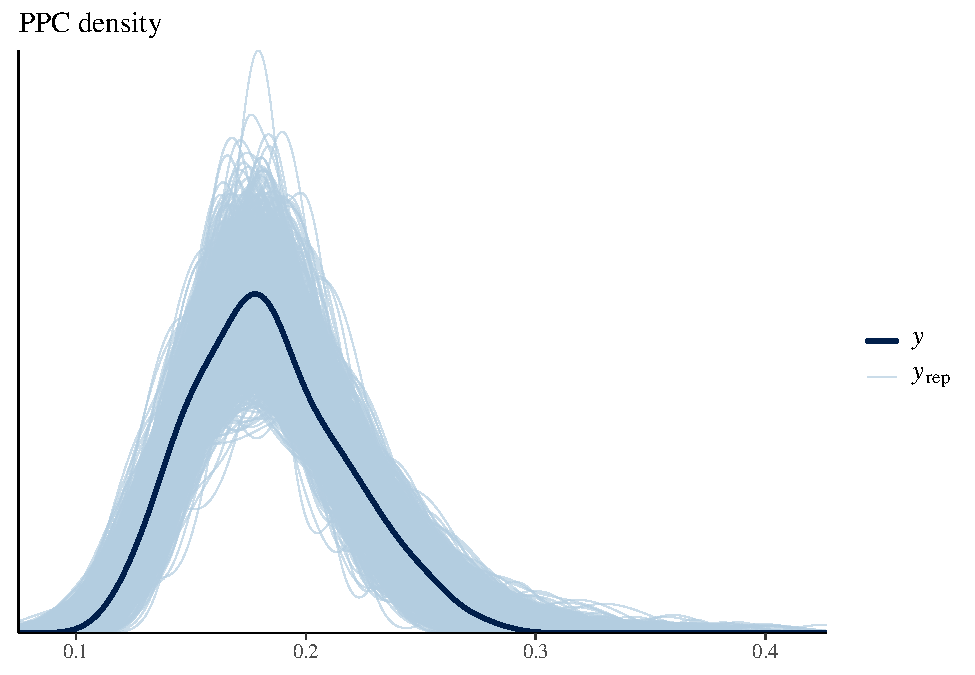
\includegraphics[keepaspectratio]{Untitled_files/figure-latex/unnamed-chunk-8-1.pdf}}
\caption{PPC density of 2000 predict results from posterior.}
\end{figure}

\subsection{Model Testing}\label{model-testing}

We take \(12000\) number of draws from the posterior distribution.
\#\#\# LOO-PIT QQ plot The Leave-One-Out Probability Integral Transform
Quantile-Quantile plot (LOO-PIT QQ plot) can check if the predictions
calibrated correctly and if the predictive distributions biased, which
is defined as:
\[ \mathrm{LOO\text{-}PIT}_i = P(\tilde{y}_i \le y_i |y_{-i}) .\]

Here we still use Monte Carlo method to simulate it, as:

\[
\mathrm{LOO\text{-}PIT}_i
= \frac{1}{S} \sum_{s=1}^{S} 
\mathbf{1}\!\left( \tilde{y}_{i,-i}^{(s)} \le y_i \right)
\] where \(S\) is the number of posterior draws. We will use it to check
if our posterior is under or over dispersion, the good model's PIT plot
should be flat over \(Uniform(0,1)\). For our model, the PIT histogram
(Figure 4) is flat everywhere except probability near 0.55 and 0.8,
which are acceptable by the randomness of MCMC method. A U-shape (points
over dot line at two tails) in PIT plots means overestimates variance,
it doesn't appear in our plot gives evidence of our choices on variables
and likelihood family.

\pandocbounded{\includegraphics[keepaspectratio]{Untitled_files/figure-latex/unnamed-chunk-9-1.pdf}}
\#\#\# Coverage rate and Errors

Table 3 shows the coverage rate of \(95\%\) and \(50\%\) predicted
intervals, which means \(98\) and \(52\) individuals' real \(\beta\)
value is inside the intervals. The MAE and RMSE are both relatively
small.

\begin{longtable}[]{@{}lr@{}}
\caption{Testing table}\tabularnewline
\toprule\noalign{}
Metric & Value \\
\midrule\noalign{}
\endfirsthead
\toprule\noalign{}
Metric & Value \\
\midrule\noalign{}
\endhead
\bottomrule\noalign{}
\endlastfoot
95\% predictive interval coverage & 0.980 \\
50\% predictive interval coverage & 0.510 \\
Mean Absolute Error & 0.023 \\
Root Mean Square Error & 0.029 \\
\end{longtable}

\section{Example}\label{example}

Now we will apply our model on an individual example: A \(70\) year old
female (weight: \(70\)kg, height: \(160\)cm) is arrested after being
stopped by the police while driving. She provides a blood sample to the
police \(2\) hours after her arrest which gives a reading of Ct =
\(0.15\)g/kg. The legal limit is x = \(0.47\)g/kg.

Since there is no `drinking time' data here, we will use a simplified
model with only `sex', `height', `weight' variables. We have
standardized height and weight by using sample's mean and variance.

As figure 7 shows, this is the posterior density of \(C_0\) calculated
by presicted posterior density of \(\hat{\beta}\) the dot line is the
legal limit \(C_0 = 0.47\), it can be seen that most density is larger
than \(0.47\), so obviously the 70 year old female is over the drink
driving limit.

\begin{figure}
\centering
\pandocbounded{\includegraphics[keepaspectratio]{Untitled_files/figure-latex/unnamed-chunk-11-1.pdf}}
\caption{Posterior Predictive Distribution of C\_0, message=FALSE,
warning=FALSE, with limit C\_0 = 0.47 (dot line).}
\end{figure}

To make the result clear, it is better to give Table 4 to the courts and
illustrate:

\begin{center}
There is $91.4\%$ probability that the 70 year old female is over the drink driving limit, with both mean, median and mode value over the limit.
\end{center}

The results also show that the original method is not reasonable since
\(2.5\%\) percentile is over-conservative even in this case.

\begin{longtable}[]{@{}lr@{}}
\caption{Example results}\tabularnewline
\toprule\noalign{}
Statistic & Value \\
\midrule\noalign{}
\endfirsthead
\toprule\noalign{}
Statistic & Value \\
\midrule\noalign{}
\endhead
\bottomrule\noalign{}
\endlastfoot
Mean & 0.560 \\
Median & 0.553 \\
Mode & 0.542 \\
2.5\% & 0.439 \\
25\% & 0.510 \\
75\% & 0.604 \\
97.5\% & 0.715 \\
P(C\_0 \textgreater{} 0.47) & 0.913 \\
\end{longtable}

\section{\texorpdfstring{Widmark's Equation and
\(V_d\)}{Widmark's Equation and V\_d}}\label{widmarks-equation-and-v_d}

\section{Further research:}\label{further-research}

casual effect: biased data selection, (e.g.~inner correlations between
sex and height)

\subsection{Variable Description}\label{variable-description}

\begin{itemize}
\tightlist
\item
  how many observations do we have? where we get the resourse,
  reference? explain each variables in table
\end{itemize}

The variables identified for the analysis are demographic and
physiological characteristics from the tested individuals after drinking
alcohol. Our variable selection is informed by their established
relevance to human liver metabolic function, especially sex, age, weight
and height are included due to the significant influence on liver
metabolism.

\begin{itemize}
\tightlist
\item
  Sex: Biological sex of the individual, male or female
\item
  Age:
\item
  Weight\\
\item
  Height
\item
  Beta60:
\item
  Co:
\end{itemize}

Page, Participant number, FigureOnPage, Sample Type\ldots{} clearly
inrevelant,

Maximum BAC/BrAC,BAC peak time 也可推断为无关factor
与police预测受测者驾驶中酒精浓度的目标不同

\subsection{Prelimary analysis}\label{prelimary-analysis}

\begin{itemize}
\tightlist
\item
  initial formula: explain beta60 + - motivation to improve?
\end{itemize}

variable correlations? Why? hypothesis needed? why 2.5 quantiles?

\section{Model selection regarding key variable
`beta60'}\label{model-selection-regarding-key-variable-beta60}

\subsection{Advantage of current
method}\label{advantage-of-current-method}

simpler model with only one parameter(beta), easier to calculate,
suitable for no dataset situations

\#Limitation our model limit data collected reason - cannot reflect the
real world model reason other reason: variables

\#Reference 空腹低 长期饮酒高CTP2E1活性高 性别肝脏大小 药物抑制酒精代谢
测两次血预测beta
如果司机坐在方向盘后面没有被捕,瑞典的交警通常会提交间隔约1小时采集的双重血液样本。假设存在吸收后下降阶段和零阶动力学操作,每个采样时间的平均结果可用于计算酒精的消除率。根据长期调查酒后驾车案件的经验,第一个血液样本通常在逮捕后60分钟获得,这取决于该人被逮捕的全国地点以及是否有医生或护士抽血。
\url{https://www.sciencedirect.com/science/article/pii/S0379073810000770?via\%3Dihub}

P.Y. Kwo, V.A. Ramchandani, S. O'Connor, D. Amann, L.G. Carr, K.
Sandrasegaran, K.K. Kopecky, T.K. Li Gender differences in alcohol
metabolism: relationship to liver volume and effect of adjusting for
body mass Gastroenterology, 115 (1998), pp.~1552-1557

\end{document}
